\section{Мета роботи}
Набути навичок та закріпити знання при виконанні операцій на
мультисписках та нелінійних списках.

\section{Хід роботи}
Для варіантів завдань 1 – 13 розробити програму, що створює список
списків (нелінійний список). Передбачити такі функції:

\begin{itemize}
  \item додавання елементів у список та підсписок (при додаванні елемента
  у головний список додається і відповідний підсписок);
  \item видалення елементів зі списку та підсписків (при видаленні
  елемента з головного списку видаляється і пов’язаний з ним підсписок);
  \item видача вмісту списків та підсписків у консоль;
  \item видалення списків;
\end{itemize}

\textbf{Моє завдання:} \\

Список: Будівельні фірми. 

Підсписок: Перелік зданих об’єктів.

\clearpage
\subsection{Реалізація списку будівельних фірм на базі списку з лабораторної 7}
Було реалізовано такі методи: \textit{ініціалізація списку, видалення списку, вивід списку та його підсписку у консоль}.

\begin{lstlisting}[style=customc]
#include "lab8_list.h"

#include <stdio.h>
#include <stdlib.h>
#include <string.h>

// init building list
BuildingFirm *create_building_firm(const char *name)
{
  BuildingFirm *firm = (BuildingFirm *)malloc(sizeof(BuildingFirm));
  if (!firm)
  {
    perror("Cannot allocate memory for BuildingFirm!");
    exit(EXIT_FAILURE);
  }
  strcpy(firm->name, name);
  firm->sublist = NULL;
  return firm;
}

// destroy building list
void destroy_building_firm(void *data)
{
  BuildingFirm *firm = (BuildingFirm *)data;
  if (firm->sublist)
  {
    destroy_linked_list(&firm->sublist, free);
  }
  free(firm);
}

void print_sublist_item(const void *data)
{
  printf("  %s\n", (const char *)data);
}

void print_building_firm(const void *data)
{
  const BuildingFirm *firm = (const BuildingFirm *)data;
  printf("\033[32m Building Firm:\033[0m %s\n", firm->name);

  if (firm->sublist)
  {
    printf("  Objects:\n");
    print_linked_list(firm->sublist, print_sublist_item);
    puts("");
  }
  else
  {
    printf("  No objects.\n");
  }
}
\end{lstlisting}

\clearpage
\subsection{Реалізація лабораторної програми}
Було створено список фірм з заповненою інформацією про них, проведено операції додавання та видалення до списку.

\begin{lstlisting}[style=customc]
#include <stdio.h>
#include <stdlib.h>
#include <string.h>

#include "general_utils.h"
#include "lab8_list.h"

int compare_firms(const void *a, const void *b)
{
  return strcmp(((BuildingFirm *)a)->name, (const char *)b);
}

void task1()
{
  Node *firms = NULL; // firms list

  char firm1[] = "Avantazh";
  char firm2[] = "Kharkiv Bud Development";
  char firm3[] = "StroyCity";
  char firm4[] = "MegaBuild";
  char firm5[] = "UrbanBuilders";

  insert_head_linked_list(&firms, create_building_firm(firm1));
  insert_head_linked_list(&firms, create_building_firm(firm2));
  insert_head_linked_list(&firms, create_building_firm(firm3));
  insert_head_linked_list(&firms, create_building_firm(firm4));
  insert_head_linked_list(&firms, create_building_firm(firm5));

  BuildingFirm *builderA = (BuildingFirm *)firms->data;
  insert_head_linked_list(&builderA->sublist, strdup("Block of flats"));
  insert_head_linked_list(&builderA->sublist, strdup("Office Building"));
  insert_head_linked_list(&builderA->sublist, strdup("Skyscraper 'Bluetech'"));
  insert_head_linked_list(&builderA->sublist, strdup("Apartment Complex"));

  BuildingFirm *builderB = (BuildingFirm *)firms->next->data;
  insert_head_linked_list(&builderB->sublist, strdup("Shopping Mall"));
  insert_head_linked_list(&builderB->sublist, strdup("Business Center"));
  insert_head_linked_list(&builderB->sublist, strdup("Residential Complex 'SunCity'"));

  BuildingFirm *builderC = (BuildingFirm *)firms->next->next->data;
  insert_head_linked_list(&builderC->sublist, strdup("Cultural Center"));
  insert_head_linked_list(&builderC->sublist, strdup("Sports Arena"));
  insert_head_linked_list(&builderC->sublist, strdup("Concert Hall"));

  BuildingFirm *builderD = (BuildingFirm *)firms->next->next->next->data;
  insert_head_linked_list(&builderD->sublist, strdup("Luxury Apartments"));
  insert_head_linked_list(&builderD->sublist, strdup("High-Tech Skyscraper"));
  insert_head_linked_list(&builderD->sublist, strdup("Eco-Friendly Office"));

  BuildingFirm *builderE = (BuildingFirm *)firms->next->next->next->next->data;
  insert_head_linked_list(&builderE->sublist, strdup("Urban Park"));
  insert_head_linked_list(&builderE->sublist, strdup("Family Housing Complex"));
  insert_head_linked_list(&builderE->sublist, strdup("Community Center"));

  highlightText("ALL AVAIBLE FIRMS\n", "blue");

  print_linked_list(firms, print_building_firm);

  highlightText("DELETING FIRMS: Avantazh, StroyCity, UrbanBuilders\n", "blue");
  delete_node_linked_list(&firms, firm1, compare_firms, destroy_building_firm);
  delete_node_linked_list(&firms, firm3, compare_firms, destroy_building_firm);
  delete_node_linked_list(&firms, firm5, compare_firms, destroy_building_firm);

  highlightText("ALL AVAIBLE FIRMS\n", "blue");
  print_linked_list(firms, print_building_firm);

  destroy_linked_list(&firms, destroy_building_firm);
}
\end{lstlisting}


\clearpage
\subsection{Результати роботи програми:}

\begin{figure}[h!]
    \centering
    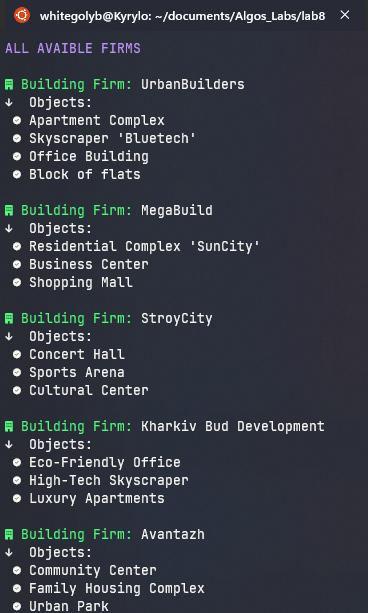
\includegraphics[width=13cm]{reports/algos/lab8/assets/1.jpeg}
    \caption{Створення та заповнення списку фірм}
\end{figure}

\begin{figure}[h!]
  \centering
  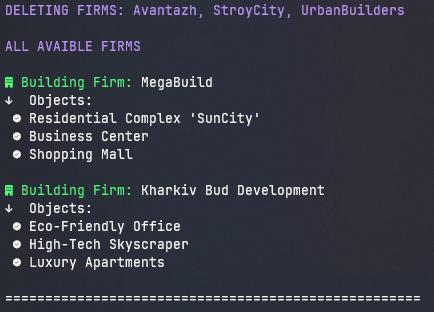
\includegraphics[width=15cm]{reports/algos/lab8/assets/2.jpeg}
  \caption{Видалення фірм зі списку та його повторне виведення на екран}
\end{figure}

\clearpage
\section{Висновки}
  В ході виконання лабораторної роботи було розроблено список фірм який складається з кастомних списків (створених на базі мого перевикористовуваного списку) та які зберігають дані профірму а також мають додаткой підсписок з її об’єктами. Успішно реалізовано операції: виведення, додавання, видалення елементів списку.



